\documentclass[../dissertation.tex]{subfiles}
\begin{document}
Now that gradient flow equation and tangent-point energy are introduced,
one can formalise the process of untangling a tangled curve:

\begin{definition}[Curve Untangling Process]
    Given a parameterised curve $\gammabf:M \times T \rightarrow \mathbb{R}^3$ over an interval $M$ and time domain $T$,
    denote the following initial value problem as \textbf{curve untangling process}:
    \begin{align}
        \frac{\partial \gammabf}{\partial t} &= - \grad_{\mathcal{X}} \mathcal{E}_{\beta}^{\alpha} (\gammabf) - \grad_{\mathcal{X}} \mathcal{C} (\gammabf) 
        \label{equ: Curve Untangling Process}
        \\
        \gammabf(s;0) &= \gammabf_0 (s)
        \label{equ: Initial Curve}
    \end{align}
    where 
    \begin{itemize}
        \item $\gammabf_0 (s)$ is the parameterisation of the initial (tangled) curve (prescribed at $t=0$)
        \item $\mathcal{E}_{\beta}^{\alpha}$ is the tangent-point energy (See (\ref{equ: Tangent-Point Energy}))
        \item $\mathcal{C}$ is additional constraint energy to control behaviour of curve untangling process.
    \end{itemize}
\end{definition}



\subsection{Discretisation for Numerical Computation}
Solving (\ref{equ: Curve Untangling Process}), (\ref{equ: Initial Curve}) analytically is challenging.
Rather, we aim to acquire a numerical solution.
Assume for simplicity that the curve of interest is simple closed.\footnote{
    We may assume that the function definition of $\gammabf:M \rightarrow \mathbb{R}^3$ extends to $\gammabf: \mathbb{R} \rightarrow \mathbb{R}^3$ by periodicity.
}

\subsubsection{Discretisation of Curve}
We start by discretising the initial curve $\gammabf_0$ by taking $N$ points on a curve as shown in Figure \ref{fig: Discretization of Curve}.
Represent the initially discretised curve in the form of multidimensional array (or a matrix for specific time step index):
$\Gammabf^0 = \left( \xbf_0^0, \xbf_1^0, \cdots, \xbf_{N-1}^0 \right) \in \mathbb{R}^{3 \times N}$,
and the discretised curve at subsequent time step $k \in \mathbb{N} \cup \left\{ 0 \right\}$ as $\Gammabf^k = \left( \xbf_0^k, \xbf_1^k, \cdots, \xbf_{N-1}^k \right) \in \mathbb{R}^{3 \times N}$.
Since we restrict our attention to a simple closed curve, it is convenient to extend the indexing rule by:
\begin{equation}
    \xbf_{i}^k = \xbf_{r\left( i,N \right)}^k \hspace{1cm} \text{where } r\left( i,N \right) = \text{(remainder of } i \div N \text{)}
\end{equation}
so that $\xbf_N^k = \xbf_{0}^k$, $\xbf_{N+1}^k = \xbf_{1}^k$, etc.

Define (right) operator $[\cdot]:\mathbb{R}^{3 \times N} \rightarrow \mathbb{R}$ such that for array $T \in \mathbb{R}^{3 \times N}$,
%$\Gammabf^k: \mathbb{Z} \rightarrow \left\{ \xbf_0^k, \xbf_1^k, \cdots, \xbf_{N-1}^k \right\}$ as:
\begin{equation*}
    T[i] \coloneqq T \ebf_{r\left( i,N \right)}
\end{equation*}
where $\ebf_i$ is the $i$\textsuperscript{th} canonical vector.
With this operator, one could write
\begin{equation}
    \Gammabf^k [i] = \xbf_{r\left( i, N \right)}^k = \xbf_i^k
\end{equation}
analogous to $\gammabf = \gammabf(s;t)$ being a parameterised curve, which is a vector-valued function.

Finally, denote by $e_{i}^k$ for the (undirected) edge with vertex pair $\left( \xbf_i^k, \xbf_{i+1}^k \right)$.

\subsubsection{Discretisation of Tangent-Point Energy}
In order to acquire numerical solution, one must also be able to numerically compute the tangent-point energy.
For this, we pose the energy quadrature $E_{\beta}^{\alpha} \left( \Gammabf^k \right)$ of the following form:
\begin{equation}
    \mathcal{E}_{\beta}^{\alpha} \left( \gammabf \left( \cdot, t \right) \right) \coloneqq
    \iint_{M^2} k_{\beta}^{\alpha} (\gammabf_x, \gammabf_y) \intd \gamma_x \intd \gamma_y
    \approx
    E_{\beta}^{\alpha} \left( \Gammabf^k \right) \coloneqq
    \sum_{i, j \in \left\{ 0, \cdots, N-1 \right\}} K_{\beta}^{\alpha} \left( i, j \right) \norm{e_i^k} \, \norm{e_j^k}
    \label{equ: Energy Approximation Form}
\end{equation}
where
$K_{\beta}^{\alpha}$ is an approximation of tangent-point kernel $k_{\beta}^{\alpha}$ (which is specified at (\ref{equ: Kernel 4-point})), 
and $\norm{e_i^k}$ is the length of edge $e_i^k$, that is, $\norm{e_i^k} = \norm{\xbf_i^{k+1} - \xbf_i^k}$.
Note that $\Gammabf^k$ is a polygonal curve, for which tangent-point energy (\ref{equ: Tangent-Point Energy}) is not well-defined due to locally non-integrable contributions from vertices:

\begin{figure}[tbp]
    \centering
    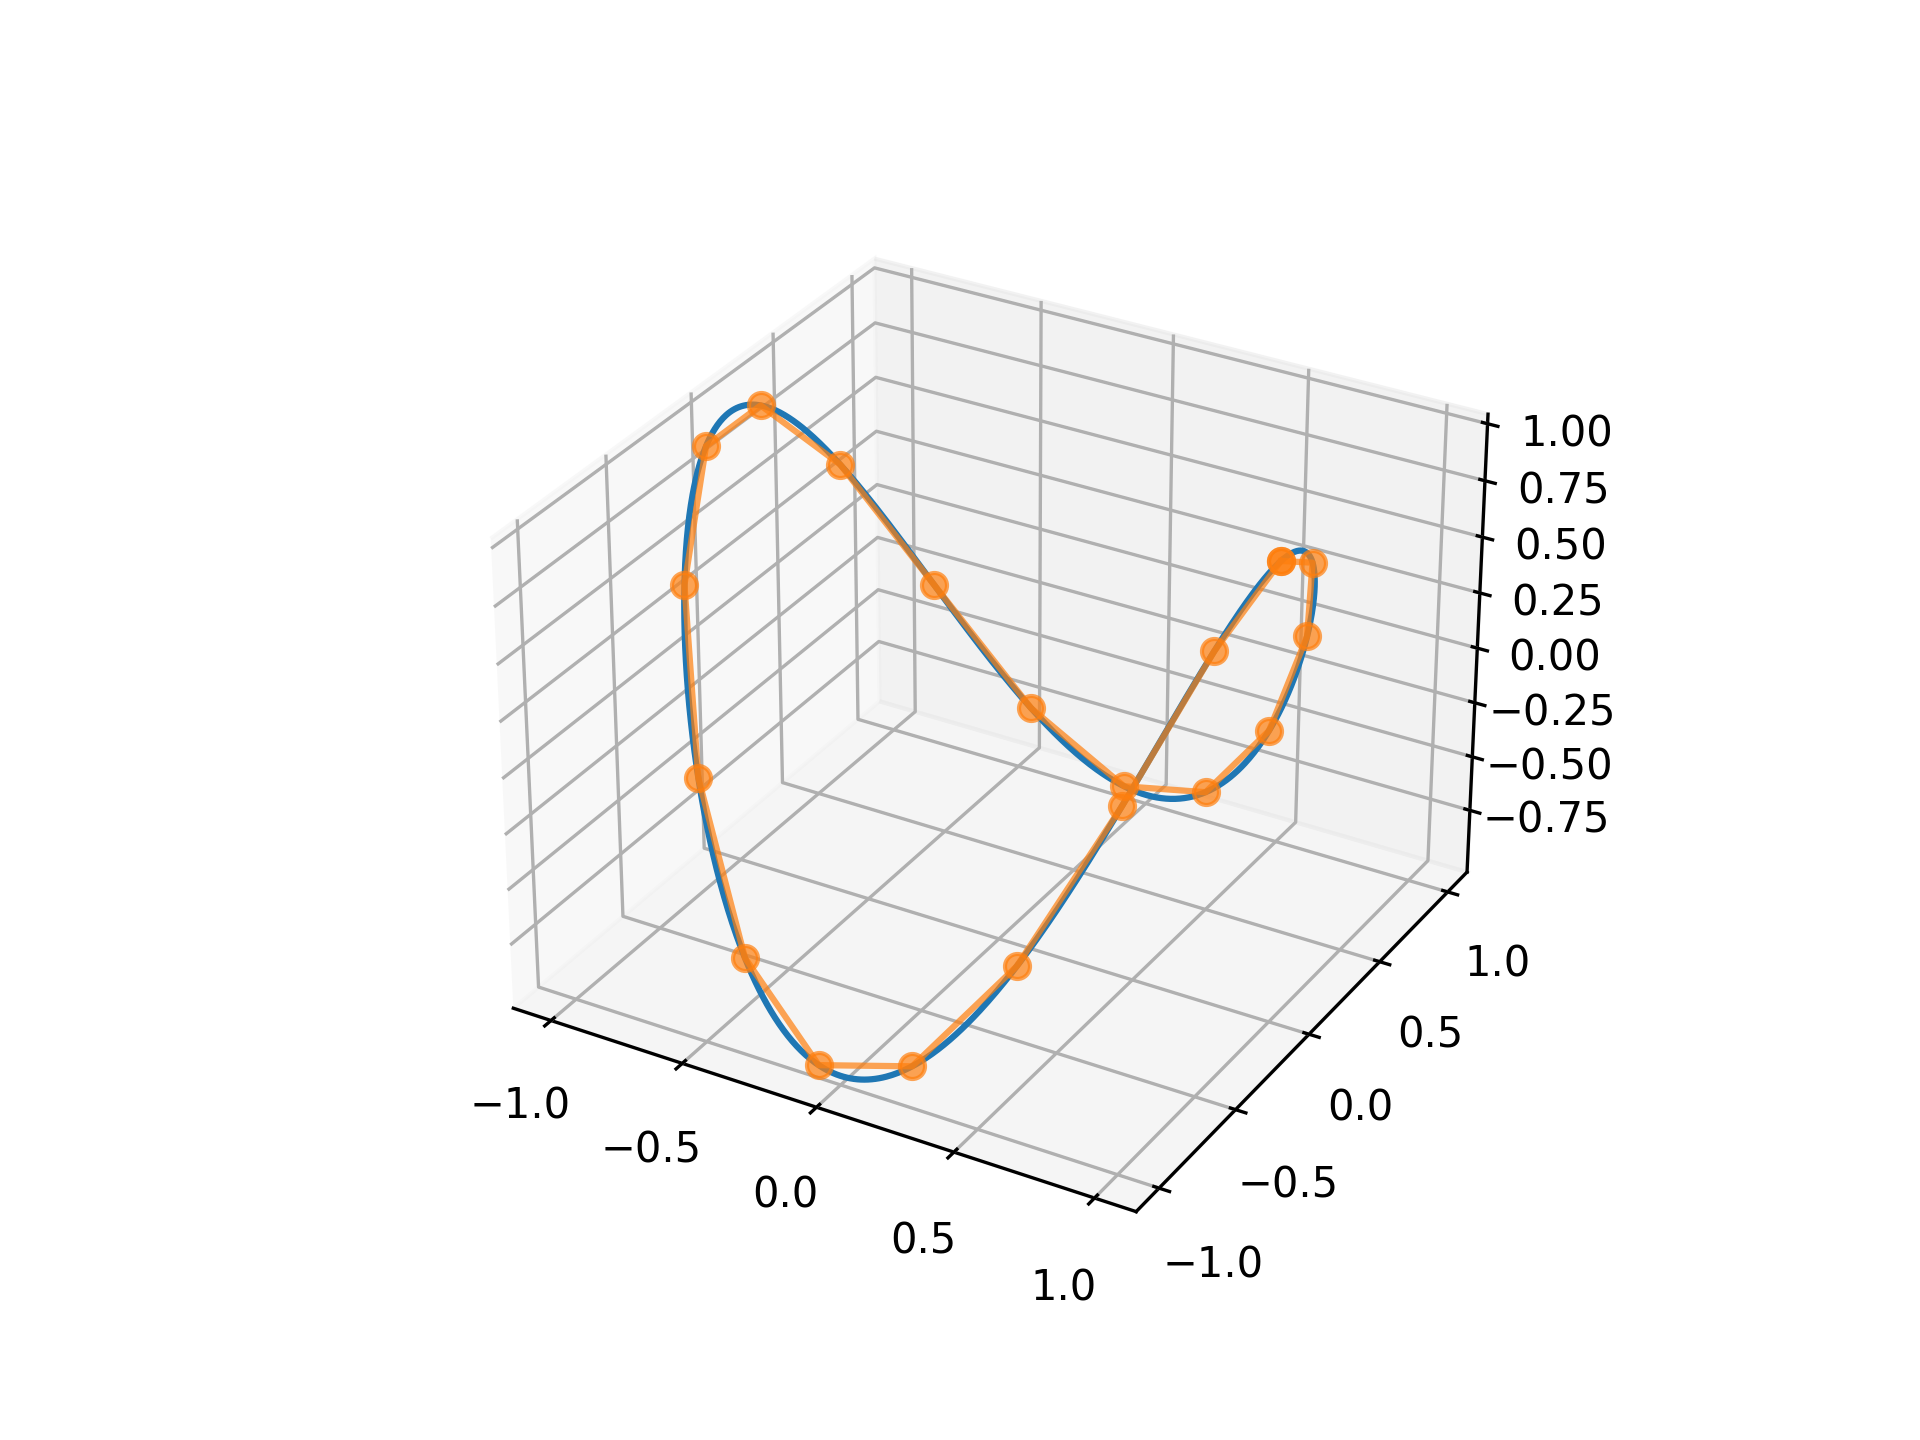
\includegraphics[width=0.8\textwidth]{sections/discretizationImgs/discretization}
    \caption{Discretisation of a simple closed curve by sampling the points along the curve.}
    \label{fig: Discretization of Curve}
\end{figure}

One way to resolve the issue is to ``ignore'' the adjacent edge contribution\cite{YSC2021} in the energy quadrature $E_{\beta}^{\alpha}$ as shown in Figure \ref{fig: Energy discretization by ignoring adjacent edges}.
The justification is that as we take a finer mesh ($N$ sufficiently large), the product of edge lengths ($\norm{e_i}\norm{e_j}$) should tend to zero sufficiently fast, resulting in approximation of the energy for the smooth curve, which did not have vertices resulting in local non-integrability in the first place.
\begin{figure}[tbp]
    \centering
    \begin{subfigure}[b]{0.75\textwidth}
        \centering
        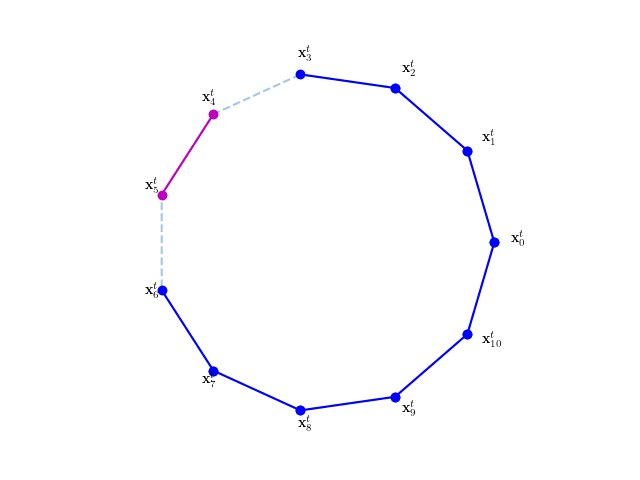
\includegraphics[width=\textwidth]{sections/unknottingCurveImgs/energyDiscretization1}
        \caption{For a chosen edge $e_i^k$, ignore the two adjacent edges $e_{i-1}^k$, $e_{i+1}^k$.
            In the limit as $N \rightarrow 0$, because the edge lengths tend to zero,
            the discrepancy between the quadrature and the analytical value of the energy is expected to tend to zero.
                }
        \label{fig: Energy discretization by ignoring adjacent edges}
    \end{subfigure}
    \par\bigskip
    \begin{subfigure}[b]{0.75\textwidth}
        \centering
        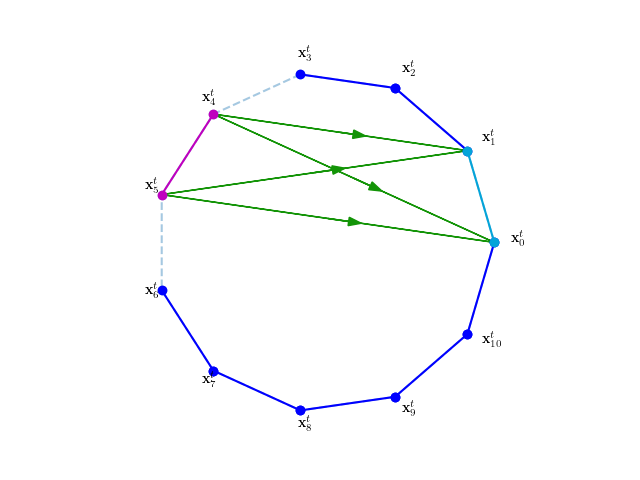
\includegraphics[width=\textwidth]{sections/unknottingCurveImgs/energyDiscretization2}
        %\caption{Tangent-point kernel is approximated by 4-point quadrature $K_\beta^\alpha (i, j)$ defined as (\ref{equ: Kernel 4-point}).}
        \caption{Tangent-point kernel is approximated by 4-point quadrature defined as (\ref{equ: Kernel 4-point}).}
        \label{fig: Tangent-point kernel approximation}
    \end{subfigure}
    \caption{Quadrature for approximation of tangent-point energy.}
\end{figure}

It still remains to sensibly approximate the kernel $k_{\beta}^{\alpha} (\gammabf_x, \gammabf_y) \approx K_{\beta}^{\alpha} (i, j)$.
One sensible approximation is to use the following 4-point quadrature\cite{YSC2021}.
\begin{multline}
    K_{\beta}^{\alpha} (i, j) \coloneqq \frac{1}{4} \biggl( k_{\beta}^{\alpha} \left( \xbf_i^k, \xbf_j^k, \Tbf_i^k \right)
        + k_{\beta}^{\alpha} \left( \xbf_i^k, \xbf_{j+1}^k, \Tbf_i^k \right) \\
        + k_{\beta}^{\alpha} \left( \xbf_{i+1}^k, \xbf_j^k, \Tbf_i^k \right)
        + k_{\beta}^{\alpha} \left( \xbf_{i+1}^k, \xbf_{j+1}^k, \Tbf_i^k \right)
    \biggr)
    \label{equ: Kernel 4-point}
\end{multline}
where $\Tbf_{i}^k \coloneqq \frac{\xbf_{i+1}^k - \xbf_i^k}{\norm{\xbf_{i+1}^k - \xbf_i^k}}$ approximates the tangent vector to the curve at $\gammabf_x$.
(See Figure \ref{fig: Tangent-point kernel approximation}.)

Putting (\ref{equ: Energy Approximation Form}) and (\ref{equ: Kernel 4-point}) together,
one can write the \textbf{tangent-point energy quadrature} as:
\begin{equation}
    E_{\beta}^{\alpha} \left( \Gammabf^k \right) \coloneqq \sum_{\substack{i, j \in \left\{ 0, \cdots, N-1 \right\} \\ r \left( i-j,N \right) > 1}} K_{\beta}^{\alpha} (i,j) \norm{e_i^k} \, \norm{e_j^k}
    \label{equ: Tangent-Point Energy Quadrature}
\end{equation}
where $r\left( i-j,N \right)$ is the geodesic distance between $i$ and $j$ in modulo $N$,
characterising the avoidance of adjacent edges on simple closed polygonal curve.
For discussion of quadratures for nonclosed curves, see appendix \ref{sct: Other Homeomorphism Classes}.


\subsubsection{Derivative Operators Discretised Curve}
For discrete curve, the (forward and backward) first derivative operators (\ref{equ: Curve Gradient Operator}) transforms to operator for $U \left( \Gammabf^k \left[ \cdot \right] \right): \left\{ 0, 1, \cdots, N-1 \right\} \rightarrow \mathbb{R}$ characterised by:
\begin{align}
    \curvenabla_{\Gammabf^k}^{+} U \left( \Gammabf^k \left[ i \right] \right) &= \frac{U \left( \Gammabf^k \left[ i+1 \right] \right) - U \left( \Gammabf^k \left[ i \right] \right)}{\norm{\Gammabf \left[ i+1 \right] - \Gammabf \left[ i \right]}} \Tbf_i^k\\
    \curvenabla_{\Gammabf^k}^{-} U \left( \Gammabf^k \left[ i \right] \right) &= \frac{U \left( \Gammabf^k \left[ i \right] \right) - U \left( \Gammabf^k \left[ i-1 \right] \right)}{\norm{\Gammabf \left[ i \right] - \Gammabf \left[ i-1 \right]}} \Tbf_{i-1}^k
\end{align}
and analogously with second derivative operator:
\begin{align}
    \curvelaplacian_{\Gammabf^k} U \left( \Gammabf[i] \right)
    &=
    \frac{\frac{U \left( \Gammabf^k [i+1] \right) - U\left( \Gammabf^k [i] \right)}{\norm{\Gammabf^k \left[ i+1 \right] - \Gammabf^k \left[ i \right]}} - \frac{U \left( \Gammabf^k [i] \right) - U \left( \Gammabf^k \left[ i-1 \right] \right)}{\norm{\Gammabf^k[i] - \Gammabf^k[i-1]}}}{\frac{1}{2}\norm{\Gammabf^k \left[ i+1 \right] - \Gammabf^k \left[ i-1 \right]}}
    \label{equ: Discrete Curve Laplacian} \\
    &= 
    %\frac{\frac{U_{i+1} - U_{i}}{\norm{e_i}} - \frac{U_{i} - U_{i-1}}{\norm{e_{i-1}}}}{\norm{f_i}} \\
    %&= 
    \frac{\norm{e_i} U_{i-1} - \left( \norm{e_{i-1}} + \norm{e_{i}} \right) U_i + \norm{e_{i-1}} U_{i+1} }{\norm{e_{i-1}} \, \norm{e_i} \, \norm{f_i}} \\
    &= 
    \frac{1}{\norm{e_{i-1}} \, \norm{e_i} \, \norm{f_i}}
    \begin{pmatrix}
        \norm{e_i} & -\left( \norm{e_{i-1}} + \norm{e_i} \right) & \norm{e_{i-1}}
    \end{pmatrix}
    \begin{pmatrix}
        U_{i-1} \\
        U_i \\
        U_{i+1}
    \end{pmatrix}
    \label{equ: Discrete Curve Laplacian Matrix Form}
\end{align}
where one defines $f_i \coloneqq \frac{1}{2} \left( \Gammabf^k \left[ i+1 \right] - \Gammabf^k \left[ i-1 \right] \right)$
and $U_{i} \coloneqq U\left( \Gammabf^k \left[ i \right] \right)$.

However, inverting the Laplacian is troublesome, as it is equivalent to inverting a singular matrix as stated in the following lemma.
\begin{lemma}
    \label{lemma: Curve Laplacian is Singular}
    The matrix capturing curve Laplacian $\curvelaplacian_{\Gammabf^k}$ for closed discrete curve $\Gammabf^k$ is singular.
\end{lemma}
\begin{proof}
    The matrix $L$ for $\curvelaplacian_{\Gammabf^k}$ for closed discrete curve $\Gammabf^k$ has the form:
    \begin{equation*}
        L \coloneqq
        \begin{pmatrix}
            * & * &   &   &   & & * \\
            * & * & * &   &   & &  \\
            & * & * & * &  &  &   \\
            &   & \ddots  & \ddots & \ddots &  & \\
            &   &   & *  &  * & * & \\
            &  & &  & *  & *  & * \\
            * &   & &  &   & *  & *
        \end{pmatrix}
    \end{equation*}
    To show that $L$ is singular, it is sufficient to show that there is a nontrivial solution $\xbf$ to $L \xbf = \zerobf$.
    Since rows follow from (\ref{equ: Discrete Curve Laplacian Matrix Form}),
    observe that the rows sum to zero.
    Hence, one can spot such nontrivial solution $\xbf = \left( 1, 1, \cdots, 1 \right)^T$.
\end{proof}
In order to proceed, one needs to ``regularise'' the Laplacian to make it invertible as in section \ref{sct: Example: Euler Scheme in Other Spaces}.

\subsubsection{Finite Difference Scheme of Curve Untangling Process}
Based on (\ref{equ: Curve Untangling Process}), one writes the following finite difference scheme:
\begin{equation}
    \mathcal{D}_{t} \Gammabf^{k} = -\Grad_{X} E_{\beta}^{\alpha} (\Gammabf^k) - \Grad_{X} C \left( \Gammabf^k \right) \hspace{1cm} \text{for } k=0,1,\cdots
    \label{equ: Finite Difference Scheme for Curve Untangling Process}
\end{equation}
where $\mathcal{D}_t$ is the finite difference operator over time,
$\Grad_{X}$ is discrete equivalent\footnote{Worth noting that $\Grad_X:\mathbb{T} \rightarrow \mathbb{T}$ where $\mathbb{T}$ is a set of arrays of certain shape; $\Grad_X$ maps arrays to arrays of the same shape.}  of $\grad_{\mathcal{X}}$ on discrete inner product space $X$ (which may be omitted in the notation),
$E_{\beta}^{\alpha}$ is the tangent-point energy quadrature defined as (\ref{equ: Tangent-Point Energy Quadrature}),
and $C$ is the discretised version of the constraint energy $\mathcal{C}$ (See section \ref{sct: Constraint Energy}).
Often times, however, it is easier to construct finite difference scheme directly from (\ref{equ: Curve Untangling Process}) after some simplification,
rather than attempting to use (\ref{equ: Finite Difference Scheme for Curve Untangling Process}) directly.
Note that because similar operations are done for each point vector, this is a parallelisable task.
For the simplest scheme, one could take the forward difference operator characterised as $\mathcal{D}_t \Gammabf^k[i] \coloneqq \frac{\Gammabf^{k+1}[i] - \Gammabf^{k}[i]}{\Delta T}$.

\subsection{Example: $L^2$ Explicit Euler Scheme}
Now we visit the simplest concrete numerical scheme for curve untangling process.
Assume for now scale-invariance by taking parameters $\alpha$ and $\beta$ to satisfy $\beta = \alpha+2$ (See lemma \ref{lemma: Scale-Invariance}).

In $L^2$, $\grad_{L^2} \mathcal{E}_{\beta}^{\alpha} \left( \gammabf \right)$ is simply the ``first-order perturbation'' as in (\ref{equ: L2 Gradient Explicit Form}).
Discrete equivalent is the $\ell^2$ space,
where one may justify this by noting that first-order perturbation in a curve is analogous to perturbing each of the point on its discretisation.
 %$\Grad_{\ell^2} = \nabla_{\Gammabf}$.
Taking $\mathcal{D}_t$ from (\ref{equ: Finite Difference Scheme for Curve Untangling Process}) to be forward difference operator,
\begin{equation}
    \frac{\Gammabf^{k+1} - \Gammabf^k}{\Delta T} = - \Grad_{\ell^2} E_{\beta}^{\alpha} \left( \Gammabf^k \right)
    \label{equ: L2 Explicit Euler}
\end{equation}
where one could explicitly write $\Grad_{\ell^2} E_{\beta}^\alpha \left( \Gammabf^k \right)$ as
\begin{equation}
    \Grad_{\ell^2} E_{\beta}^\alpha \left( \Gammabf^k \right)
    =
    \underbrace{
        \begin{pmatrix}
            \frac{\partial}{\partial x_{1,1}} & \frac{\partial}{\partial x_{1,2}} & \cdots & \frac{\partial}{\partial x_{1,N-1}} \\
            \frac{\partial}{\partial x_{2,1}} & \frac{\partial}{\partial x_{2,2}} & \cdots & \frac{\partial}{\partial x_{1,N-1}} \\
            \frac{\partial}{\partial x_{3,1}} & \frac{\partial}{\partial x_{3,2}} & \cdots & \frac{\partial}{\partial x_{3,N-1}}
        \end{pmatrix}
    }_{\nabla_{\Gammabf^k}}
    E_{\beta}^{\alpha} \left( \Gammabf^k \right)
    \label{equ: Gradient in l2}
\end{equation}
where $x_{j,i}$ refers to the $\left( j,i \right)$ coordinate variable for $3 \times N$ array.
\begin{figure}[tbp]
    \centering
    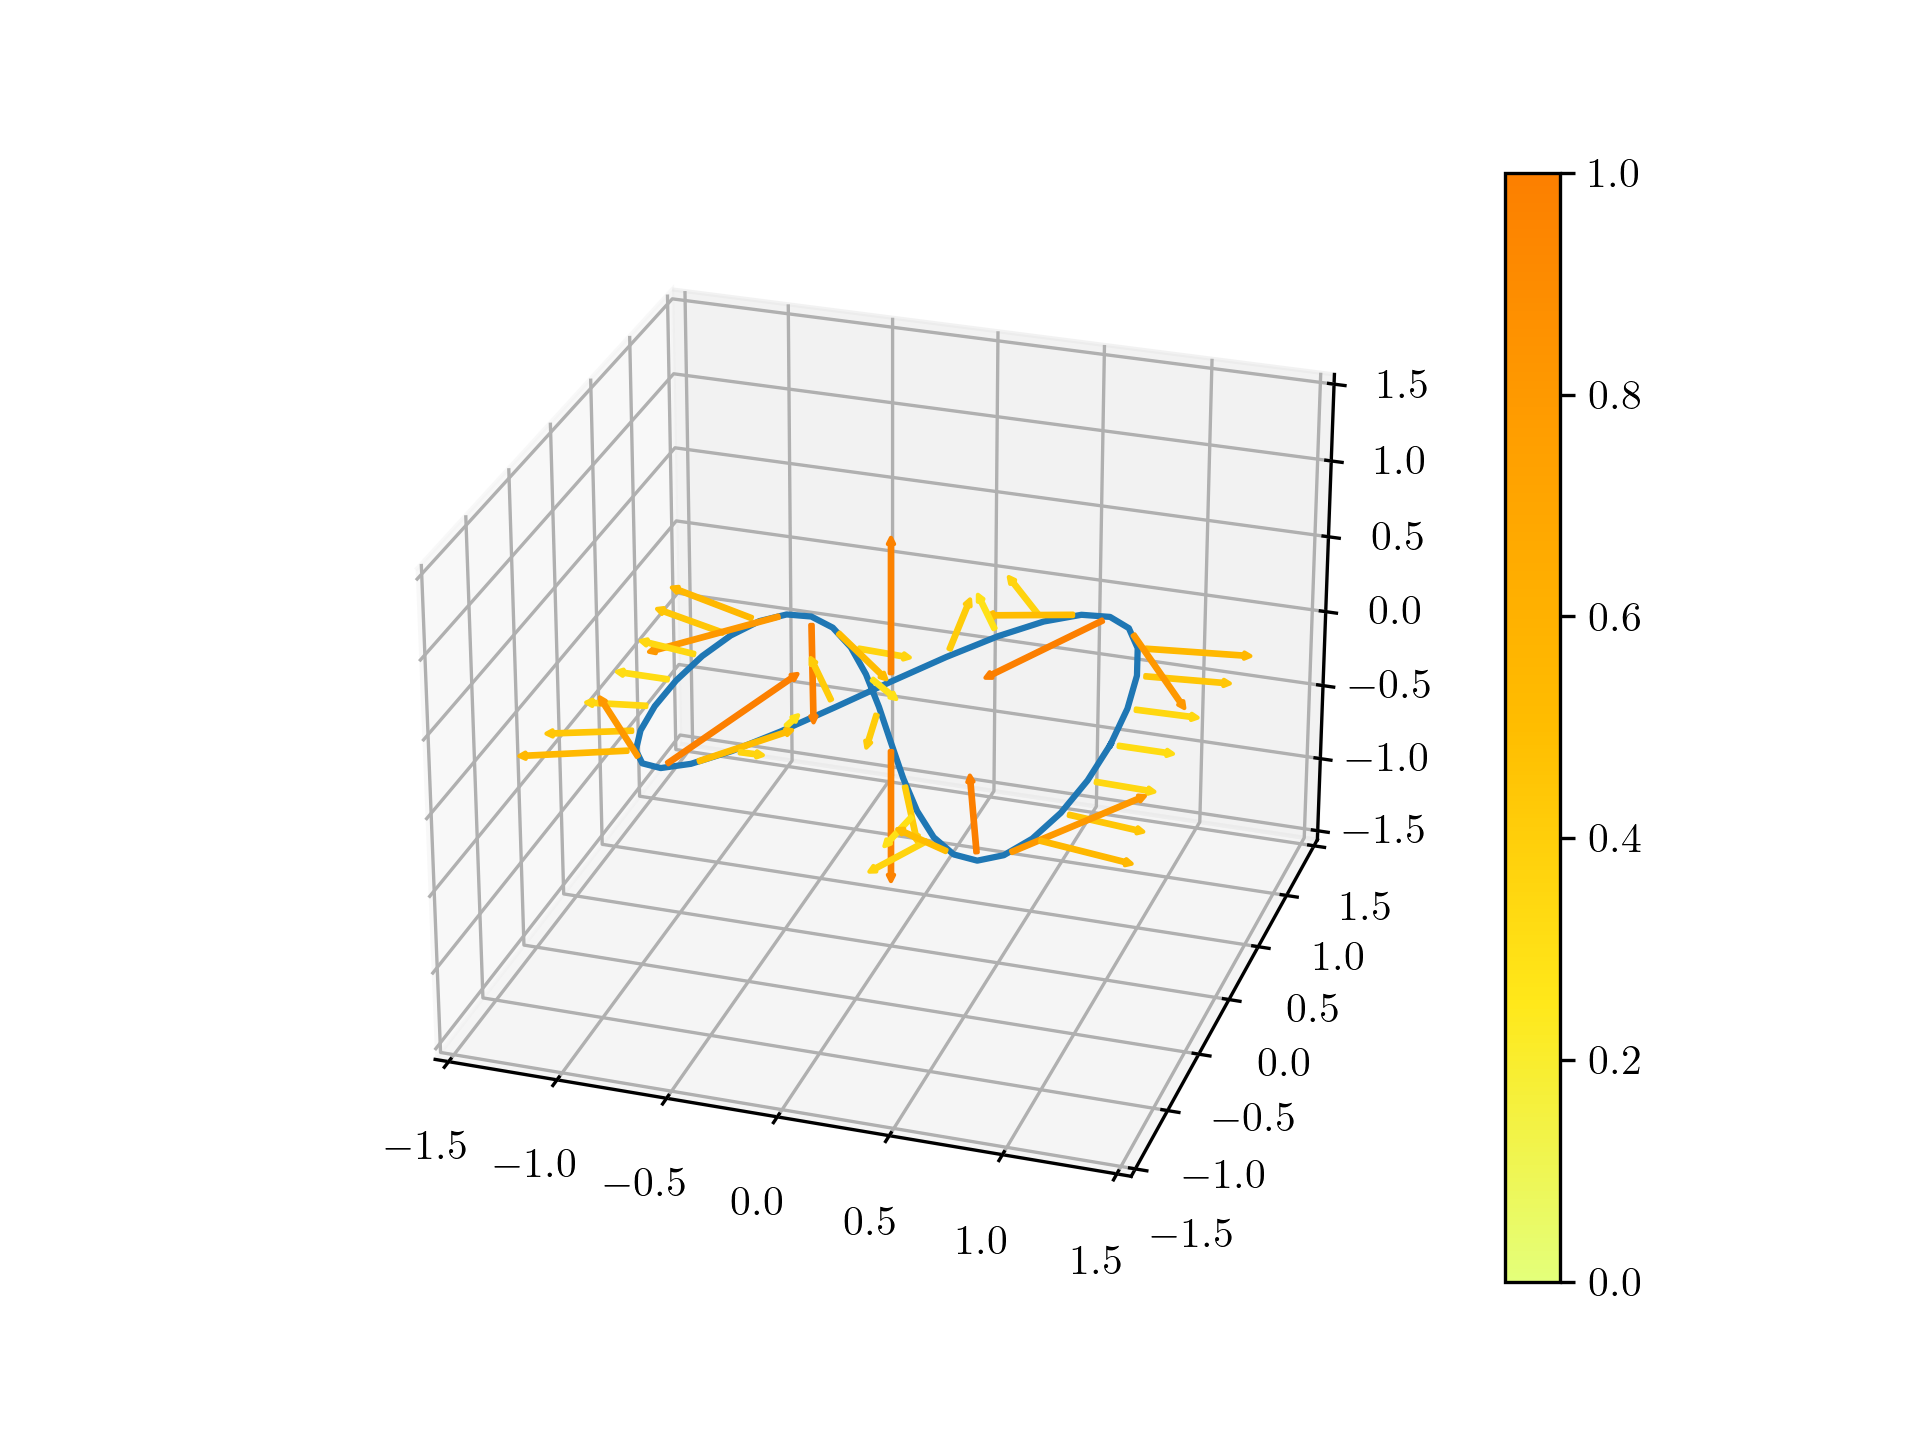
\includegraphics[width=\textwidth]{sections/unknottingCurveImgs/L2Derivative}
    \caption{$-\Grad_{L^2} \left( \Gammabf^k \right)$ which is the direction of flow of a discretised curve $\Gammabf^k$ at each point, represented by the arrows. The magnitude is represented by both color and the length of the arrows.}
    \label{fig: L2Derivative}
\end{figure}
Note that $\Grad_{\ell^2} E_{\beta}^\alpha \left( \Gammabf^k \right) \in \mathbb{R}^{3 \times N}$ is also an array of the same shape as $\Gammabf^k$,
so naturally, most arithmetics\footnote{Such as addition, subtraction, and scalar multiplication.} needed for (\ref{equ: L2 Explicit Euler}) is well-defined.
\begin{remark}
    $\Grad_{\ell^2}$ is in fact a linear operator with respect to its input, energy.
\end{remark}

One could use this exact form of $\Grad_{\ell^2} E_{\beta}^{\alpha} \left( \Gammabf^k \right)$ as given in appendix \ref{sct: Exact Gradient}, but it could be considered cumbersome (even though there are benefits to implementing this as stated in section \ref{sct: L2 Complexity}).
One could alternatively approximate $\Grad_{\ell^2} E_{\beta}^{\alpha} \left( \Gammabf^k \right)$ by central difference scheme, for example:
for $i=0,1,\cdots,N-1$ and $j = 1,2,3$,
\begin{equation}
    \ebf_j \cdot \left( \Grad_{\ell^2} E_{\beta}^{\alpha} \left( \Gammabf^k \right) [i] \right)
    =
    \frac{\partial E_{\beta}^{\alpha} (\Gammabf^k)}{\partial x_{j,i}}
    \approx
    \frac{1}{2 \Delta X} \left( 
        \bar{E}_{\beta}^{\alpha} (i)
        -
        \underaccent{\bar} E_{\beta}^{\alpha} (i)
    \right)
\end{equation}
where
\begin{align*}
    \bar{E}_{\beta}^{\alpha} (i) &\coloneqq E_{\beta}^{\alpha} \left( \left( \xbf_0, \cdots, \xbf_{i-1}, \xbf_i + \Delta X \ebf_{j}, \xbf_{i+1}, \cdots, \xbf_{N-1}\right) \right) \\
    \underaccent{\bar}{E}_{\beta}^{\alpha} (i) &\coloneqq E_{\beta}^{\alpha} \left( \left( \xbf_0, \cdots, \xbf_{i-1}, \xbf_i - \Delta X \ebf_{j}, \xbf_{i+1}, \cdots, \xbf_{N-1}\right) \right)
\end{align*}
See Figure \ref{fig: L2 Curve Unknotting} for a demonstration of curve untangling process using this $L^2$ gradient.
Note that because $L^2$ gradient flow does not take smoothness into account, this may break the assumption later of the smoothness of the curve,
which could be problematic as the tangent-point energy quadrature relied on the assumption that the discrete curve stays ``relatively smooth''.
%We will start with a demonstration with Buck-Orloff energy ($\alpha=2$, $\beta=4$), as one need not take into account of constraint energy $\mathcal{C}$ due to its scale invariance (lemma \ref{lemma: Scale-Invariance})\footnote{One could construct a similar working example for other scale-invariant tangent-point energies.}.

\begin{remark}
Notice that (\ref{equ: L2 Explicit Euler}) can be interpreted as SDM over all the coordinates on the curve!
This is consistent with the motivation of gradient flow equation given in section \ref{sct: Motivation of Gradient Flow Equation}.
\end{remark}

\begin{figure}[tbp]
    \centering
    \begin{subfigure}[b]{0.32\textwidth}
        \centering
        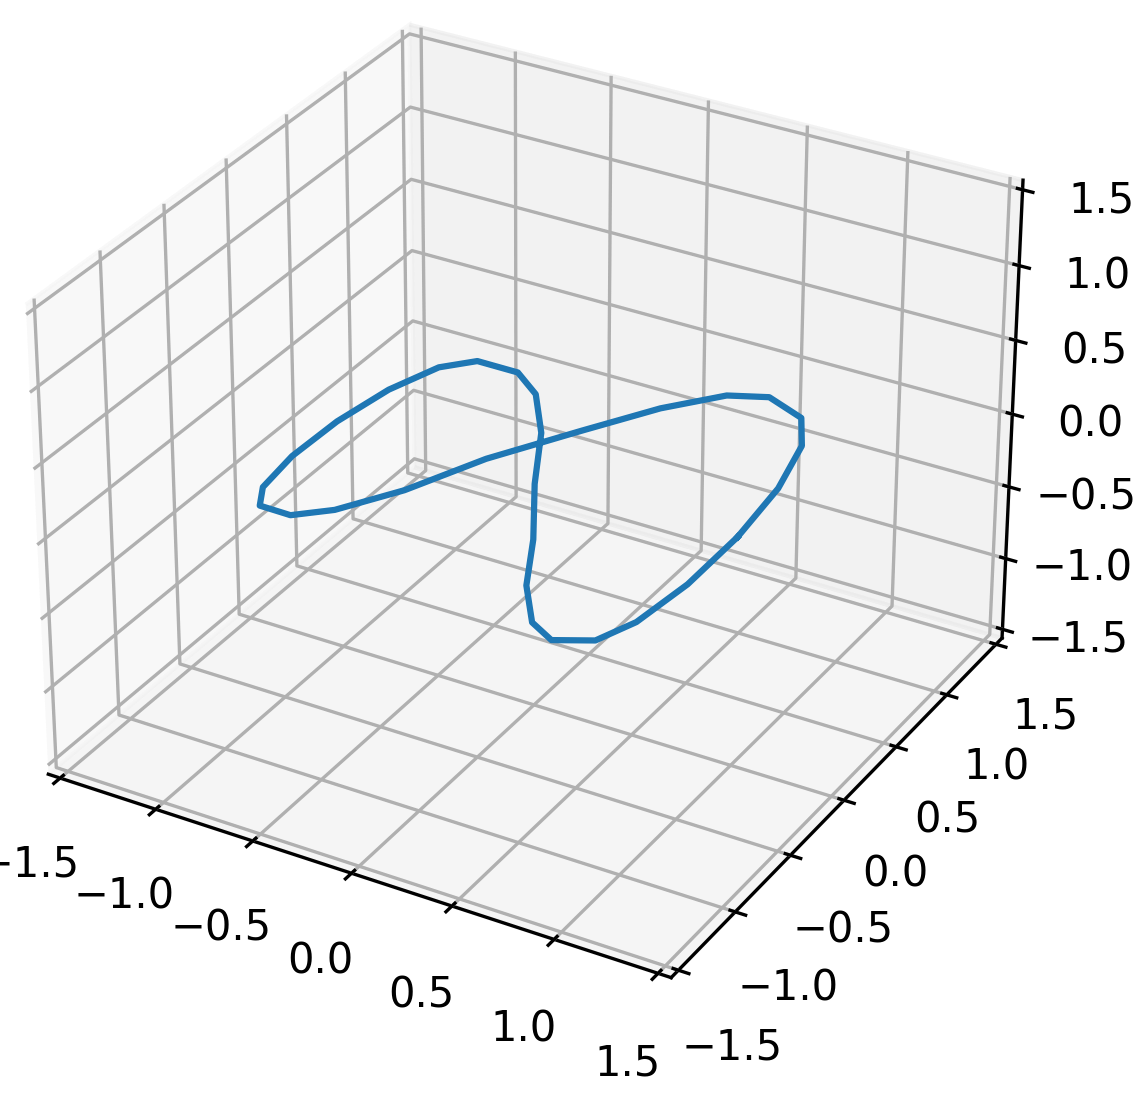
\includegraphics[width=\textwidth]{sections/unknottingCurveImgs/figure8-L2-0}
    \end{subfigure}
    \begin{subfigure}[b]{0.32\textwidth}
        \centering
        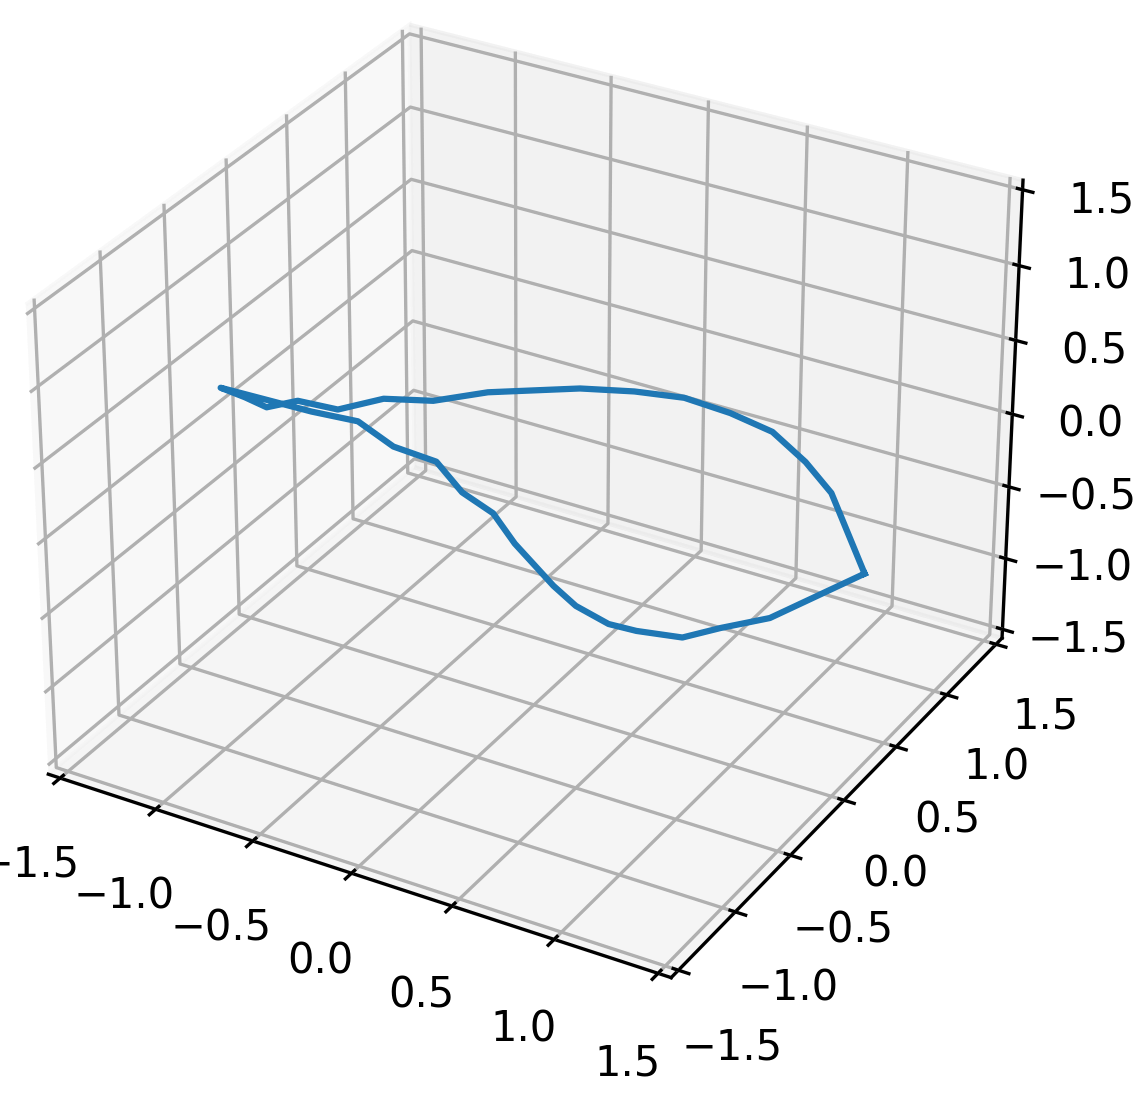
\includegraphics[width=\textwidth]{sections/unknottingCurveImgs/figure8-L2-1}
    \end{subfigure}
    \begin{subfigure}[b]{0.32\textwidth}
        \centering
        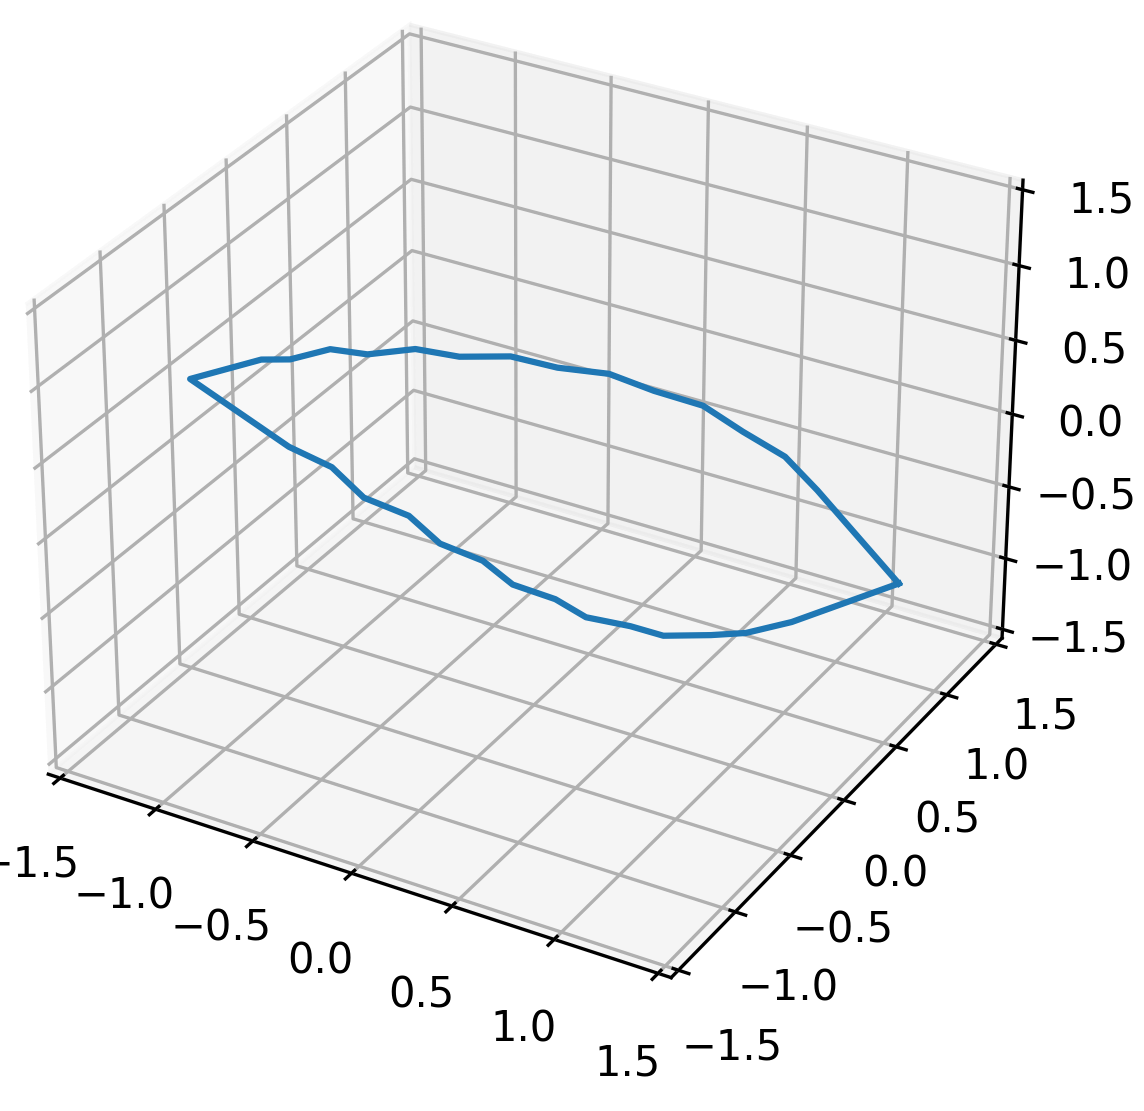
\includegraphics[width=\textwidth]{sections/unknottingCurveImgs/figure8-L2-2}
    \end{subfigure}

    \caption{$L^2$ gradient flow on a figure-eight curve. Note that there are ``sharp'' points, along with ``high frequency oscillation'' (which are undesirable or unexpected characteristics); this may be due to the fact that $L^2$ gradient flow does not take into account of the smoothness of the curve.}
    \label{fig: L2 Curve Unknotting}
\end{figure}
There is a subtlety;
there is no guarantee that the edge lengths do not grow,
which would break the assumption that the tangent-point energy quadrature is valid.
This can be mitigated by prescribing edge lengths $L_i$ using some constraint energy as in section \ref{sct: Constraint Energy}.

We now attempt the finite difference scheme with a \textit{scale-variant energy}, that is, when $\beta > \alpha + 2$. 
If one attempts the same finite difference scheme as (\ref{equ: L2 Explicit Euler})
one may observe that the curve ``grows'' in size, indefinitely.
This is due to the fact that with $\beta > \alpha + 2$,
by the virtue of lemma \ref{lemma: Scale-Invariance},
energy scales inversely proportional to its scale factor.
(See Figure \ref{fig: Scale Variant})
To use scale-variant energy, one may consider having constraint energy as part of the curve untagling process.
\begin{figure}[tbp]
    \centering
    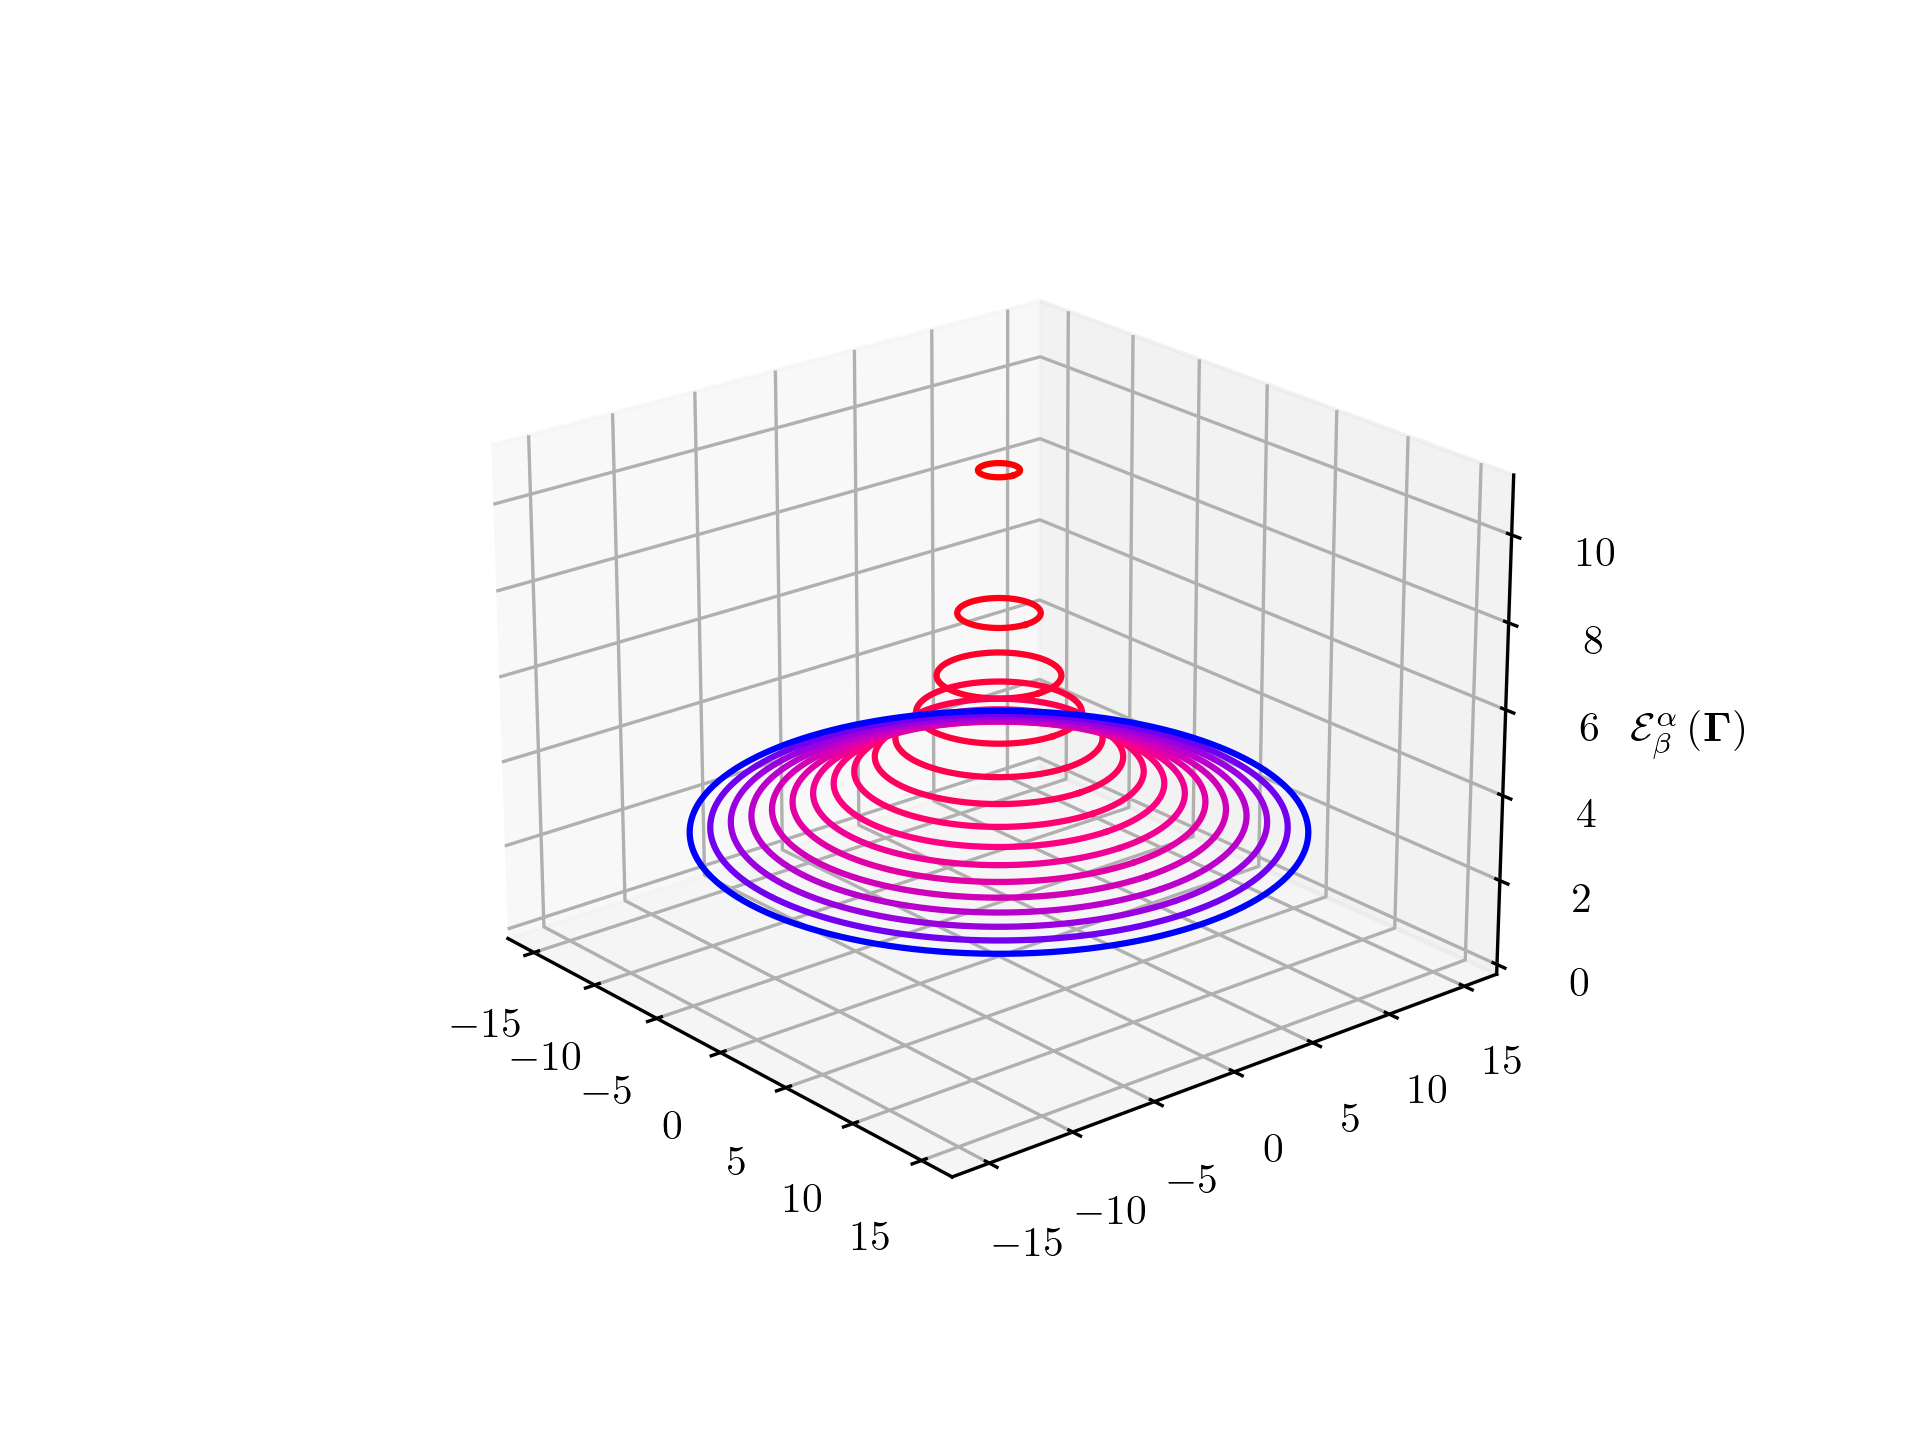
\includegraphics[width=0.85\textwidth]{sections/unknottingCurveImgs/scaleVariant}
    \caption{The height represents $\mathcal{E}_{4.5}^{2}$ for circles of different radius. Note that the energy decreases trivially by taking a larger circle.}
    \label{fig: Scale Variant}
\end{figure}
\subsubsection{Constraint Energy}
\label{sct: Constraint Energy}
From lemma \ref{lemma: Scale-Invariance} and as demonstrated in Figure \ref{fig: Scale Variant}, in the case that $\beta > \alpha + 2$,
one could trivially minimise tangent-point energy $\mathcal{E}_{\beta}^{\alpha}$ of the curve 
(and by the same logic, $E_{\beta}^{\alpha}$ of the discretised curve, albeit due to increases in edge lengths, would cease to be a ``valid'' quadrature)
by scaling the curve to infinity.
In order to avoid this phenomenon, or to change the behaviour of the flow, one may add additional energy which penalises unwanted behaviours.

Here are some examples of constraint one could take. 
(Since we are interested in numerical schemes, constraints are expressed for $C$ rather than $\mathcal{C}$.)
%\begin{itemize}
%    \item Taking $\mathcal{C} \coloneqq \lambda \int_{M} \norm{\gammabf}^{p} \intd \gamma$ adds the motivation for the curve not to stray away from the origin.
%    \item Taking $\mathcal{C} \coloneqq \lambda \left( \int_M \intd \gamma - L \right)^p$ adds the motivation for the curve to stay close to some constant arc-length $L$.
%\end{itemize}
\begin{itemize}
    \item Taking $C \left( \Gammabf^k \right) \coloneqq \lambda \sum_{i=0}^{N-1} \norm{\Gammabf^k [i]}^p$ adds the motivation for the curve not to stray away from the origin.
    \item Taking $C \left( \Gammabf^k \right) \coloneqq \lambda \left| \sum_{i=0}^{N-1} \norm{e_i} - L \right|^p$ adds the motivation for the curve to stay close to some constant arc-length $L$.
    \item Taking $C \left( \Gammabf^k \right) \coloneqq \lambda \sum_{i=0}^{N-1} \left| \norm{e_i} - L_i \right|^p$ adds the motivation for the edge lengths on the discretised curve not to deviate from prescribed edge lengths $L_i$.
\end{itemize}
%For both cases,
$\lambda \geq 0$ is the strength of the overall constraint, and
$p > 0$ is the order of ``thresholding'', where higher $p$ would lead to harsher ``thresholding''.

\subsubsection{Time Complexity}
\label{sct: L2 Complexity}
Since we expect to take $N$ to be very large, it is reasonable to consider the computational work.

If we \textit{use a difference scheme} to approximate $\Grad_{\ell^2} E_{\beta}^\alpha \left( \Gammabf^k \right)$,
for every time step, one needs to be able to evaluate $E_{\beta}^\alpha$ for a given $\Gammabf^k \in \mathbb{R}^{3\times N}$.
From (\ref{equ: Tangent-Point Energy Quadrature}),
it takes $O \left( N^2 \right)$ evaluations of the kernel.
Since the approximation for $\Grad_{L^2} E_\beta^\alpha$ requires evaluation of the energy for each point perturbed, it takes $O \left( N^3 \right)$ evaluations of the kernel for each time step. 

On the other hand, this is where doing the hard work of implementing \textit{exact gradient computation} is beneficial,
For exact gradient implementation as in appendix \ref{sct: Exact Gradient},
it takes $O \left( N \right)$ evaluations\footnote{$4 \left( N-3 \right)$ to be exact.} of the derivative of the kernel.
This implies the overall computation needed for a single step is $O \left( N^2 \right)$.

\subsubsection{Discussion of Implicit $L^2$ Euler}
A problem with explicit schemes is that, there often exists some sort of condition for stability.
This tends to be an issue particularly when using approximation of derivatives in both time and space variables.

For unconditional stability, one may attempt (fully) implicit Euler scheme, that is,
taking $\mathcal{D}_t$ in (\ref{equ: Finite Difference Scheme for Curve Untangling Process}) to be the backward difference operator,
\begin{equation}
    \frac{\Gammabf^{k} - \Gammabf^{k-1}}{\Delta T} = -\Grad_{\ell^2} E_{\beta}^{\alpha} \left( \Gammabf^k \right)
\end{equation}
This scheme is, however, nonlinear.
One needs an efficient rootfinding algorithm (such as Newton's method) to compute each time step.

Another potential scheme is the Crank-Nicolson scheme,
where one combines both explicit and implicit scheme to achieve higher order of error.

\subsection{Example: Euler Scheme in Other Spaces}
\label{sct: Example: Euler Scheme in Other Spaces}
Consider curve untangling process in $H^{-1}$.
By (\ref{equ: H-1 Gradient}), we may write $\grad_{H^{-1}} \mathcal{E}_{\beta}^{\alpha} \left( \gammabf \right) = - \curvelaplacian_{\gammabf} \left( \grad_{L^2} \mathcal{E}_{\beta}^{\alpha} \left( \gammabf \right)\right)$,
where we do not necessarily assume scale-invariance.
For the discrete equivalent, take
\begin{equation}
    \Grad E_{\beta}^{\alpha} = - \curvelaplacian_{\Gammabf^k} \left( \Grad_{l^2} E_{\beta}^{\alpha} \left( \Gammabf^k \right) \right) = - \curvelaplacian_{\Gammabf^k} \left( \nabla_{\Gammabf^k} E_{\beta}^{\alpha} \left( \Gammabf^k \right) \right)
    %= -\nabla_{\Gammabf^k} \left( \curvelaplacian_{\Gammabf^k} E_{\beta}^{\alpha} \left( \Gammabf^k \right) \right)
\end{equation}
%where the last equality is from the fact that Laplacian and gradient operators commute \cite{679160}.
Note that computing ``third derivative operator'' %$\grad \curvelaplacian$
could increase complexity of the scheme.
In fact, if one approximates the Laplacian as (\ref{equ: Discrete Curve Laplacian}), 
%$\curvelaplacian_{\Gammabf^k} E_{\beta}^{\alpha} \left( \Gammabf^k \right)\approx \frac{\bar{E}_{\beta}^{\alpha} (i) - 2 E_{\beta}^{\alpha} \left( \Gammabf^k \right) + \underaccent{\bar}E_{\beta}^{\alpha} (i)}{\Delta X^2}$,
for each time step, it takes $O \left( N^4 \right)$ evaluations of the kernel, so the scheme becomes impractical.

On the other hand, consider curve untangling process in $H^1$.
By (\ref{equ: H1 Gradient}), we write $\grad_{H^1} \mathcal{E}_{\beta}^{\alpha} \left( \gammabf \right) = - \curvelaplacian_{\gammabf}^{-1} \grad_{L^2} \mathcal{E}_{\beta}^{\alpha}$,
and
%and the discrete equivalent becomes:
(\ref{equ: Curve Untangling Process}) without constraint term can be written as:
\begin{equation}
    \frac{\partial \gammabf}{\partial t} = \curvelaplacian_{\gammabf}^{-1} \grad_{L^2} \mathcal{E}_{\beta}^{\alpha} \left( \gammabf \right)
\end{equation}
Discretising this with forward difference for time, one gets $H^1$ explicit Euler scheme:
\begin{equation}
    \left( \frac{\Gammabf^{k+1} - \Gammabf^k}{\Delta T} \right) = \curvelaplacian_{\Gammabf^k}^{-1} \nabla_{\Gammabf^k} E_{\beta}^{\alpha} \left( \Gammabf^k \right)
\end{equation}
where $\curvelaplacian_{\Gammabf^k}$ is the Laplacian as given in (\ref{equ: Discrete Curve Laplacian}),
and $\laplacian_{\Gammabf^k}$ is still the conventional gradient operator over all the coordinates of $\Gammabf^k$.
Note that by lemma \ref{lemma: Curve Laplacian is Singular}, one needs to ``regularise'' the curve Laplacian;
we do not attempt to solve for an exact $H^1$ gradient, but rather a close one.
To compute a step, one performs three steps:
\begin{enumerate}
    \item Compute $\nabla_{\Gammabf^k} E_{\beta}^{\alpha} \left( \Gammabf^k \right)$.
    \item Solve linear system $\mathcal{L} \mathcal{G}^{T} = \left( \nabla_{\Gammabf^k} E_{\beta}^{\alpha} \left( \Gammabf^k \right) \right)^T$ for $\mathcal{G} \in \mathbb{R}^{3 \times N}$
        \begin{itemize}
            \item $\mathcal{L} = \curvelaplacian_{\Gammabf^k} + cI$ is the (almost tridiagonal by (\ref{equ: Discrete Curve Laplacian Matrix Form})) matrix capturing the ``regularised'' discrete curve Laplacian $\curvelaplacian_{\Gammabf^k}$;
                %plus a constant multiple of the identity matrix;
                %without the latter,
                because curve Laplacian matrix alone is singular, the linear system would not have a unique solution,
                and the regularisation is to pick a sensible solution to the singular linear system.
            \item $c \neq 0$ is a constant such that $c$ closer to zero characterises ``more $H^1$-like flow'', at the cost of higher conditioning number.
            \item $\mathcal{G}$ represents the discrete time derivative, that is, $\mathcal{G} = \frac{\Gammabf^{k+1} - \Gammabf^k}{\Delta T}$.
        \end{itemize}
    \item Evolve by $\Gammabf^{k+1} = \left( \Delta T \right) \mathcal{G} + \Gammabf^k$.
\end{enumerate}
\begin{figure}[tbp]
    \centering
    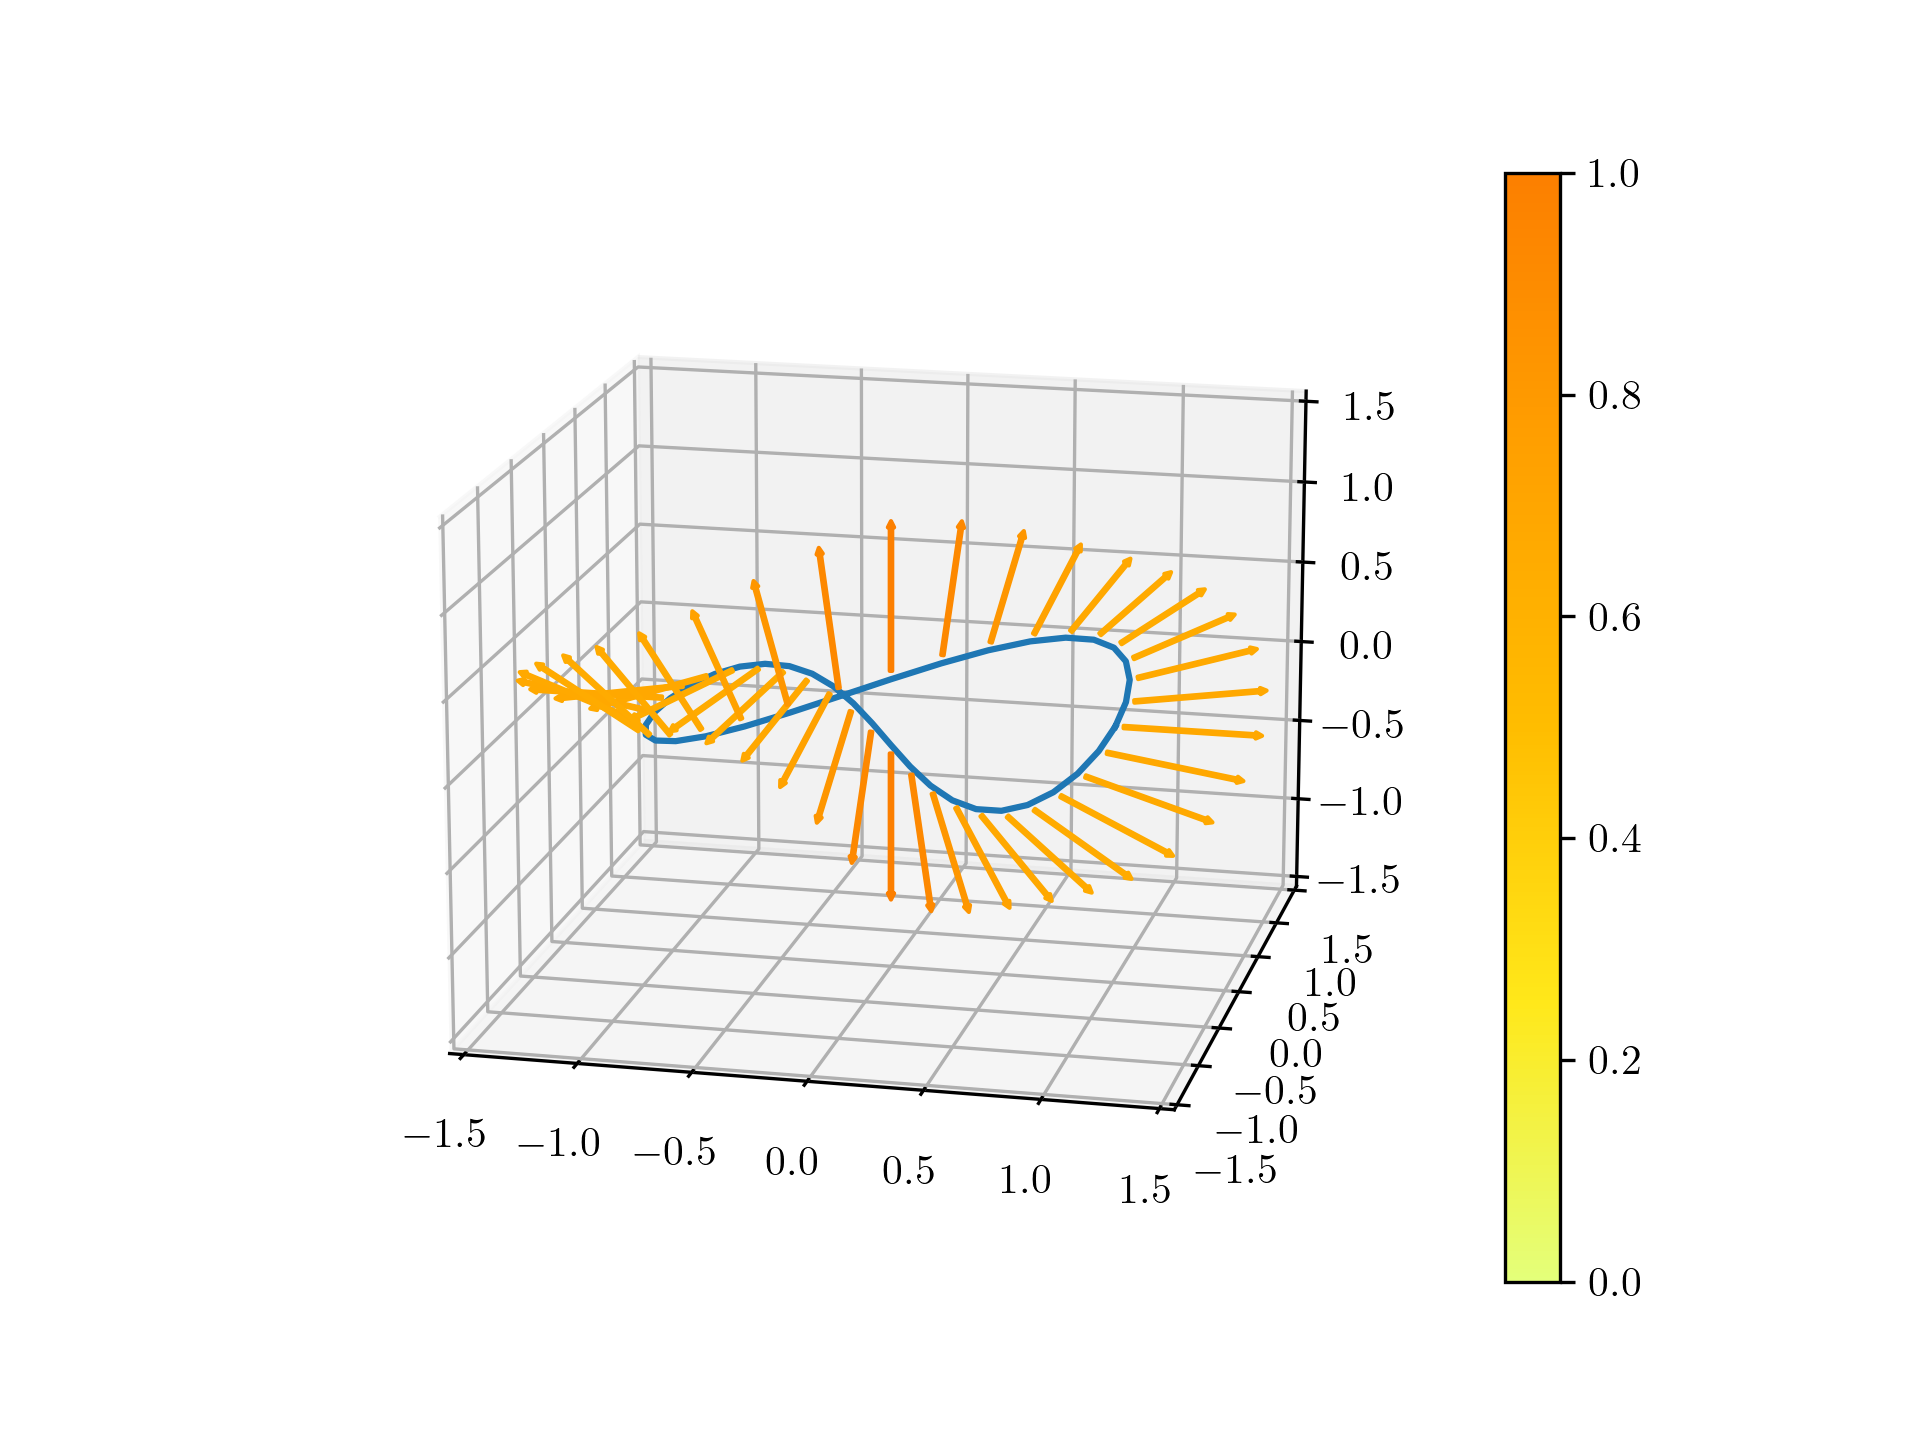
\includegraphics[width=\textwidth]{sections/unknottingCurveImgs/H1Derivative}
    \caption{$-\Grad_{H^1} E_{\beta}^{\alpha} \left( \Gammabf^k \right)$, again represented by arrows. Unlike $L^2$ gradient at Figure \ref{fig: L2Derivative}, direction of arrows are more aligned with its neighbours.}
    \label{fig: H1 Derivative}
\end{figure}
Note that the linear system $\mathcal{L} \mathcal{G}^T = \left( \nabla_{\Gammabf^k} E_{\beta}^{\alpha} \left( \Gammabf^k \right) \right)^T$ has the following structure:
\begin{equation*}
    \underbrace{
    \begin{pmatrix}
        * & * &   &   &   & & * \\
        * & * & * &   &   & &  \\
          & * & * & * &  &  &   \\
          &   & \ddots  & \ddots & \ddots &  & \\
          &   &   & *  &  * & * & \\
          &  & &  & *  & *  & * \\
        * &   & &  &   & *  & *
    \end{pmatrix}
}_{\mathcal{L} \in \mathbb{R}^{N \times N}}
\mathcal{G}^T
=
\underbrace{
\begin{pmatrix}
    * & * & * \\
    * & * & * \\
    * & * & * \\
    \vdots & \vdots & \vdots \\
    * & * & * \\
    * & * & * \\
    * & * & *
\end{pmatrix}
}_{\left( \nabla_{\Gammabf^k} E_{\beta}^{\alpha} \left( \Gammabf^k \right) \right)^T \in \mathbb{R}^{N \times 3}}
\end{equation*}
Because solving matrix equation\footnote{``Cyclic tridiagonal matrix''} $\mathcal{L} \mathcal{G}^T = \left( \nabla_{\Gammabf^k} E_{\beta}^{\alpha} \left( \Gammabf^k \right) \right)$ costs $O \left( N \right)$ by Gaussian elimination or otherwise\cite{10.1145/44164.44165},
the cost of computing $H^1$ gradient is dominated by the cost of computing $\Grad_{L^2} E_{\beta}^{\alpha} \left( \Gammabf^k \right)$.

Note that because $H^1$ takes weak derivative into account, the direction of the flow is more aligned with its neighbours as shown in Figure \ref{fig: H1 Derivative} and hence, smoother flow as shown in Figure \ref{fig: H1 Curve Unknotting}.

Also, because $H^1$ gradient operator was closer to the ``order of the differential'' of the curve,
the evolution is faster (Figure \ref{fig: Gradient Flow Energies}).
See section \ref{sct: Discussion of Fractional Sobolev Space} for a bit more detail.

\begin{figure}[tbp]
    \centering
    \begin{subfigure}[b]{0.32\textwidth}
        \centering
        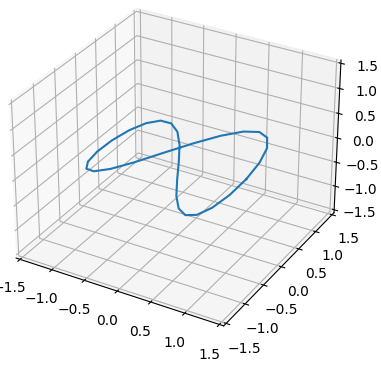
\includegraphics[width=\textwidth]{sections/unknottingCurveImgs/figure8-H1-0}
    \end{subfigure}
    \begin{subfigure}[b]{0.32\textwidth}
        \centering
        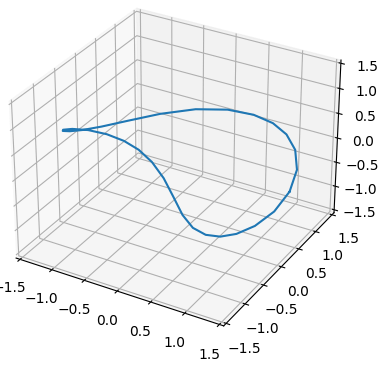
\includegraphics[width=\textwidth]{sections/unknottingCurveImgs/figure8-H1-1}
    \end{subfigure}
    \begin{subfigure}[b]{0.32\textwidth}
        \centering
        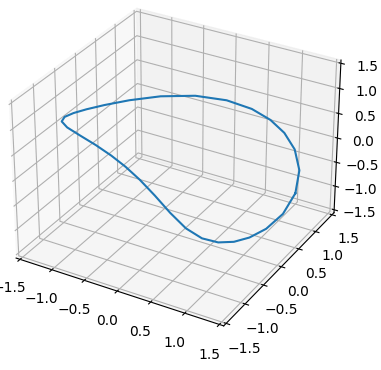
\includegraphics[width=\textwidth]{sections/unknottingCurveImgs/figure8-H1-2}
    \end{subfigure}

    \caption{$H^1$ flow on a figure-eight curve. Unlike $L^2$ flow as shown in Figure \ref{fig: L2 Curve Unknotting}, $H^1$ takes the first derivative into account, hence results in a smoother curve.}
    \label{fig: H1 Curve Unknotting}
\end{figure}

\begin{figure}[tbp]
    \centering
    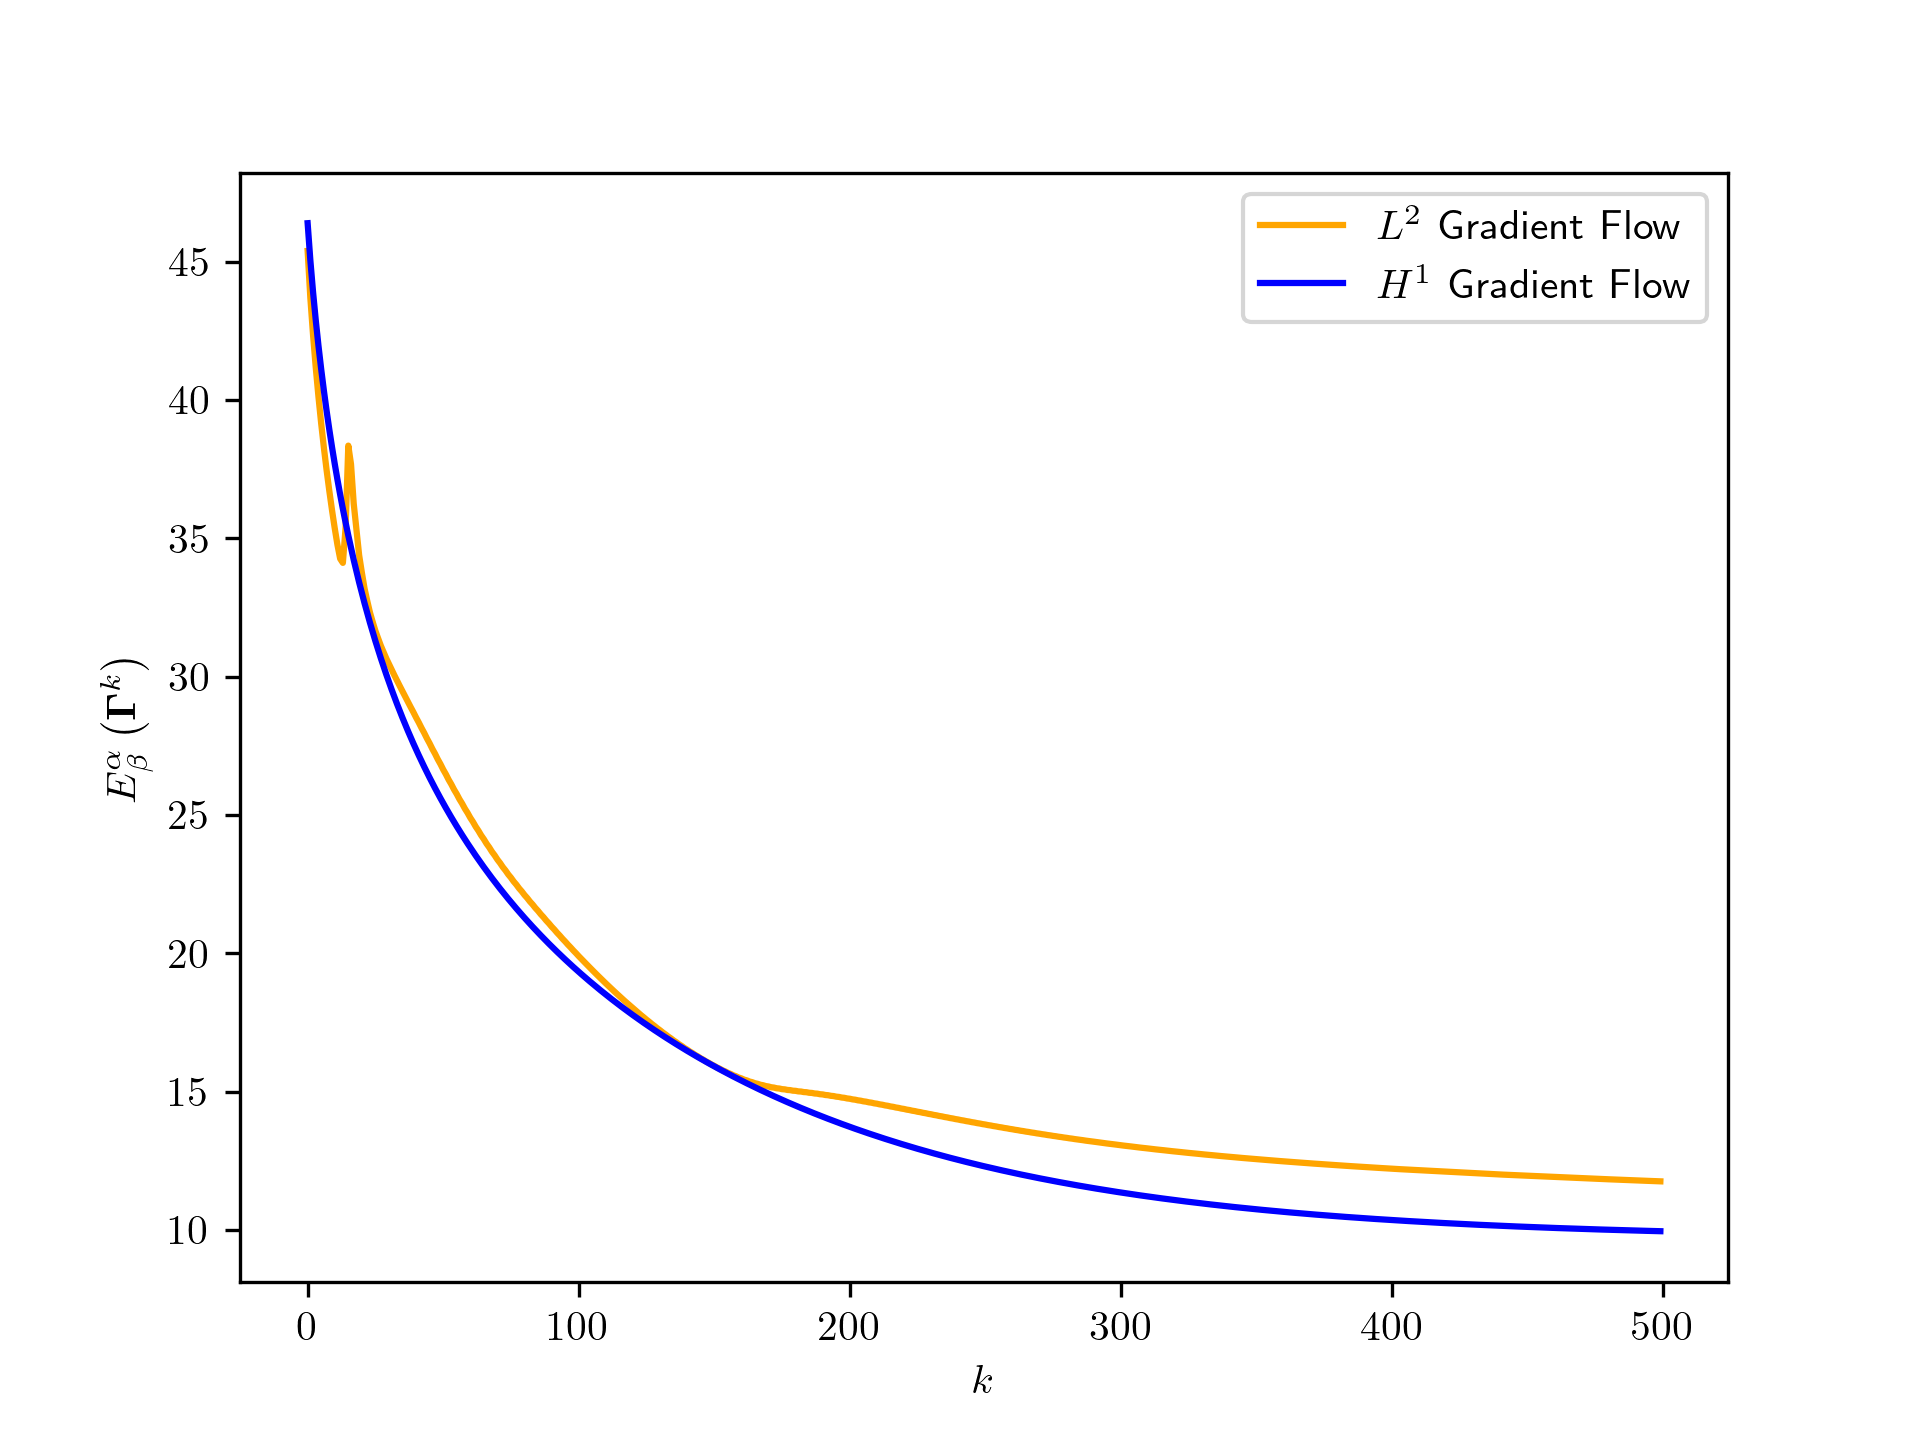
\includegraphics[width=\textwidth]{sections/unknottingCurveImgs/GradientFlowEnergies}
    \caption{Untangling the figure-eight curve. Energy of the curve evolution in each gradient flow. $H^1$ flow is slightly faster in each time step in the same conditions.}
    \label{fig: Gradient Flow Energies}
\end{figure}
\end{document}
